\section{Belægningsgrad på ortopædkirurgisk afdeling} \label{omfang}
På ortopædkirurgisk afdeling på Aalborg Universitetshospital opleves en varierende belægningsgrad for hver måned. Som tidligere nævnt i afsnit \ref{kap} ønskes en fuld kapacitetsudnyttelse, hvoraf alle sengepladser ønskes at være i brug. Belægningsgraden er antallet af de anvendte disponible senge. På \figref{maxminbelaeg} ses belægningsgraden fra år $2014$ til $2015$ på ortopædkirurgisk afdeling.\cite{SDS2015}


\begin{figure}[H]
	\flushleft 
	\centering
	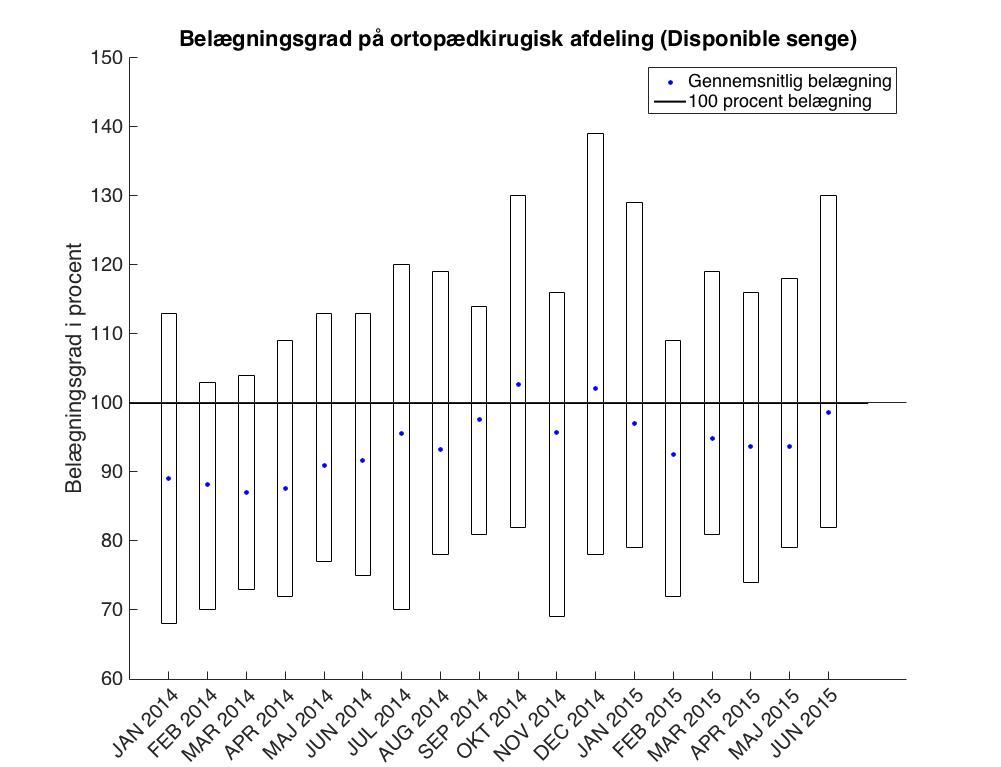
\includegraphics[scale=.45]{figures/maxminoverbelaeg.png}
	\flushleft
	\caption{\textit{Belægningsgraden på ortopædkirurgisk afdelingen på Aalborg Universitetshospital målt over $18$ måneder fra år $2014$ til $2015$. Søjlerne viser belægning ift. $100~\%$, hvortil maksimal og minimum belægning ligeledes illustreres. De blå punkter viser den gennemsnitlige belægning for hver måned.}\cite{SDS2015}}
	\label{maxminbelaeg}
\end{figure}

\noindent
Det fremgår af \figref{maxminbelaeg}, at ortopædkirurgisk afdeling oplever en belægning hhv. over og under den ønskede belægning på $100~\%$. I december måned år $2014$ ses en maksimal belægning på $139~\%$ og en minimums belægning på $78~\%$. Maksimums belægning kan indikere, at der er flere indlagte patienter end afdelingen er disponeret til, herved har afdelingen oplevet kapacitetsmangel. Minimums belægning kan indikere, at der ikke har været tilstrækkelige elektive patienter i perioder, hvilket ligeledes medfører ubalance i kapacitetsudnyttelsen. Af \figref{maxminbelaeg} er den gennemsnitlige belægning pr. måned hyppigst under $100~\%$. I oktober og december måned år $2014$ opleves dog en gennemsnitlig belægning over $100~\%$. Den gennemsnitlige belægning ses varierende mellem $90$ og $100~\%$ for de resterende måneder, hvilket kan indikere, at afdelingen oplever kapacitetsmangel i kortvarige perioder.\cite{SDS2015} 
Det fremgår ikke af den anvendte data, hvorvidt belægningen opleves i timer eller flere døgn. Dertil skal der tages forbehold for, at det ikke er angivet om det er elektive eller akutte patienter, der udgør en belægning over $100~\%$.\cite{SDS2015} 

 
For at underbygge belægningsgraden yderligere, illustrerer \figref{antaldage} antal dage pr. måned med en belægningsgrad på over $100~\%$. Denne graf er udarbejdet ud fra ortopædkirurgisk afdeling over de samme 18 måneder som \figref{maxminbelaeg}. \cite{SDS2015} 

\begin{figure}[H]
	\flushleft 
	\centering
	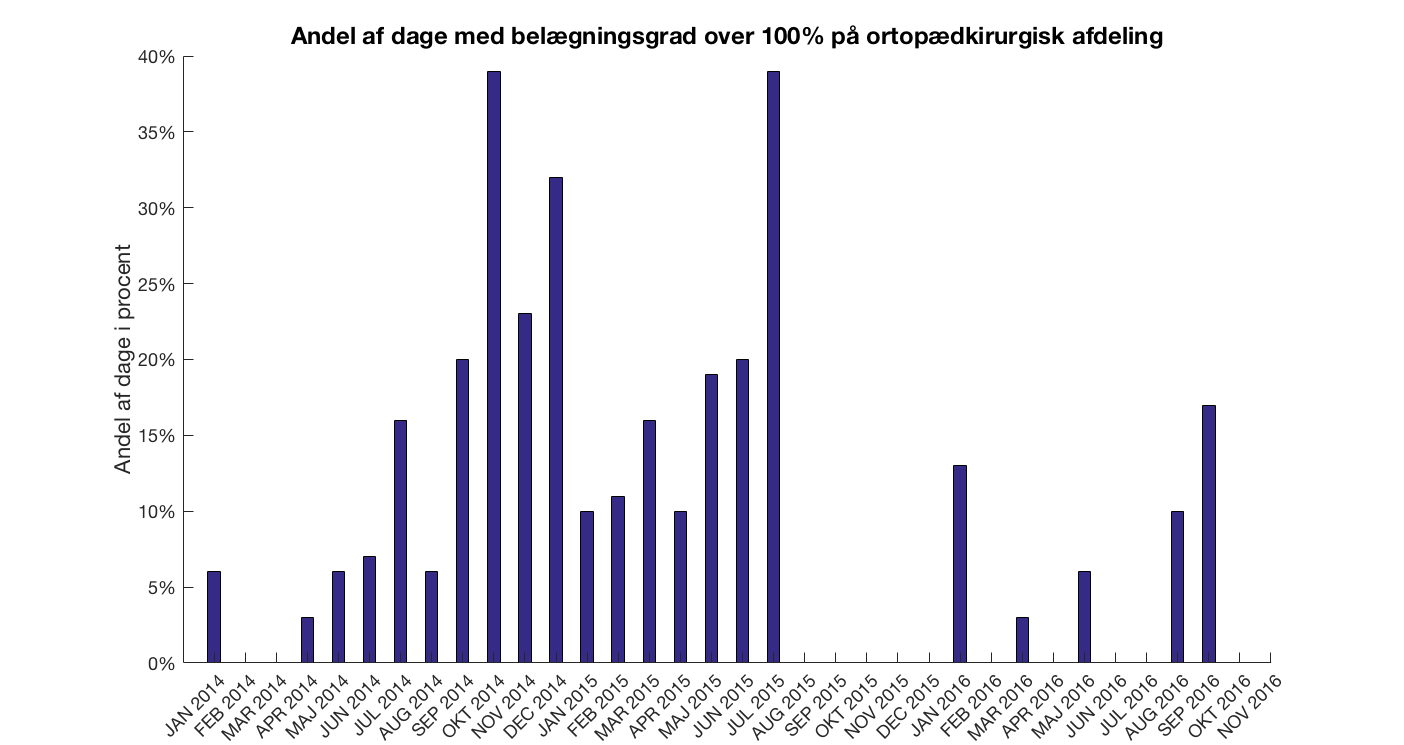
\includegraphics[scale=.4]{figures/antaldage.png}
	\flushleft
	\caption{\textit{Belægningsgrad over $100~\%$ målt i antal dage over $18$ måneder fra år $2014$ til juni $2015$ for ortopædkirugisk afdeling på Aalborg Universitetshospital.}\cite{SDS2015}}
	\label{antaldage}
\end{figure}

\noindent
Det fremgår af \figref{antaldage}, at der i oktober måned år $2014$ opleves en belægning på over $100~\%$ i $19$ dage, sammenlignes dette med oktober måned på \figref{maxminbelaeg} ses en belægning på $130~\%$. Der ses ligeledes en sammenhæng mellem de resterende måneder for de to grafer. 
Ud fra den anvendte data fremgår det ikke, hvor mange patienter, der udgør en belægningsgrad over $100~\%$, samt hvor længe de enkelte patienter er indlagt på afdelingen. Da belægningsgraden og antal dage kan variere for hver måned, anses $18$ måneder ikke som værende repræsentativ for at kunne vurdere problemets omfang. Ud fra belægningsgraden kan det dog tyde på, at en effektivisering af planlægningen af patienter på ortopædkirurgisk afdelingen vil kunne medføre en balance i kapacitetsudnyttelsen.